\chapter{Antriebsstrang}
\fancyfoot[C]{Lackner}


%% Übersicht %%%%%%%%%%%%%%%%%%%%%%%%%%%%%%%%%%%%%%%%%%%%%%%
\section{Übersicht}
Die Hauptaufgabe des Anrtiebssystems ist die Umwandlung der von dem Akkumulator zur Verfügung gestellten elektrischen Energie in die kinetische Energie. Diese tritt zuerst kreisförmig am Motor auf und wird zunächst über das direkt Getriebe umgeformt und auf die passende Drehzahl gebracht, anschließend wird die kreisförmige kinetische Energie mithilfe des Hinterrades auf die Straße übertragen und das ganze Motorrad beschleunigt. Neben dem Antrieb des Motorrades hat die Motorsteuerung noch weitere Bedeutung als Steuereinheit, diese fungiert als Bindemittel zwischen dem Human-Computer Interacting System und den elektrischen Anforderungen an das Gesamtsystem.

\subsection{Grundfunktionen des Systems}
Die geplanten Funktionen des Antriebssystems lassen sich grob in zwei Grundfunktionen einteilen.

\begin{itemize}
	\item Der Antrieb - Translation ist eine Grundfunktion eines jeden Verkehrsmittels
	\\ Durch die Umwandlung der elektrischen in kinetische Energie erfährt 
	\\ das gesamte System eine Translation.
	\item Die Steuereinheit - Steuerung und Kommunikation mit anderen Betriebsmitteln
	\\ Realisiert durch In- und Outputs, Datenübetragung mithilfe des CAN-Buses 
\end{itemize}

Nun Unterscheiden wir zwischen dem Hardware- und dem Softwareaufbau des Antriebssystems.

\newpage


%% Hardwareaufbau %%%%%%%%%%%%%%%%%%%%%%%%%%%%%%%%%%%%%%%%%%%%%%%
\section{Hardwareaufbau des Antriebssystems}
Der grudnsätzliche Hardwareaufbau des Antriebssystems lässt sich in zwei galvanisch getrennte Stromkreise und der mechanischen Umsetzung unterscheiden:

\begin{itemize}
	\item Die mechanische Umsetzung (Kraftübertragung und Montage) 
	\\ Umfasst das Getriebe und die Befestigung aller Komponenten am Rahmen
	\item Der Laststromkreis
	\\ Beinhaltet die Verbindung des Motorcontrollers mit dem Motor und dem Akkumulator.
	\item Der Steuerstromkreis
	\\ Beinhaltet alle elektrischen Verbindungen, welche mithilfe des 35-poligen
	\\ Niederleistungs-Steckers mit dem Motorcontroller verbunden sind.
\end{itemize}

%/
\begin{figure}[H]
	\begin{center}
		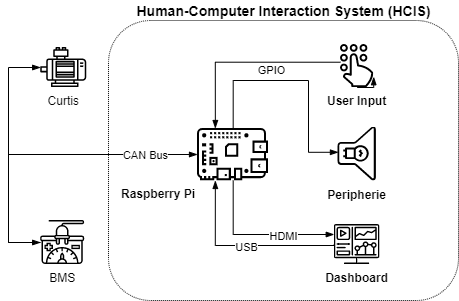
\includegraphics[scale=0.5]{figures/hcis/HCIS_Grundfunktion.png}
		\caption{Grundaufbau des Human-Computer Interaction Systems}
	\end{center}
\end{figure}

Nicht in der Abbildung dargstellt ist die Versorgung der einzelnen Komponenten, welche in dem folgenden Abschnitt noch genauer erläutert wird.


/%

\newpage

%% Mechanische Umsetzung %%%%%%%%%%%%%%%%%%%%%%%%%%%%%%%%%%%%%%%%%%%%%%% 
\subsection{Mechanische Umsetzung}
Dieser Teil des Antriebssystems wurde vollständig von Tobias Schmeisser übernommen.
--> link

%% Der Laststromkreis %%%%%%%%%%%%%%%%%%%%%%%%%%%%%%%%%
\subsection{Der Laststromkreis}
\subsection{Verbindung zum Motor}
\subsubsection{Verbindung zum Akumulator}
\subsubsection{Sonstige Komponenten}

%% Der Steuerstromkreis %%%%%%%%%%%%%%%%%%%%%%%%%%%%%%%%%%%%%%%%%%%%%%%
\subsection{Der Steuerstromkreis}
\subsubsection{Inputs}
Encoder
Throttle
Switches
\subsubsection{Outputs}
Spannungswandler
Driver



%% Softwareaufbau %%%%%%%%%%%%%%%%%%%%%%%%%%%%%%%%%%%%%%%
\section{Softwareaufbau des Antriebssystems}

%% Steuerung der In- und Outputs %%%%%%%%%%%%%%%%%%%%%%%%%%%%%%%%%%%%%%%%%%%%
\section{ Steuerung der In- und Outputs (I/O Assingment)}
\subsection{Funktionen}
\subsection{Zuweisung}


%% Drehmomentsteuerung %%%%%%%%%%%%%%%%%%%%%%%%%%%%%%%%%%%%%%%%%%%%
\section{Drehmomentsteuerung (Torquecontrol)}
\subsection{Grundfunktion}
\subsection{Parameter}

%% Kommunikation %%%%%%%%%%%%%%%%%%%%%%%%%%%%%%%%%%%%%%%%
\section{Kommunikation (CAN-Bus)}
\subsection{Grundfunktion}
\subsubsection{Parameter}
